\section{Plug and Play Generative Networks}

Shortly before this tutorial was presented at NIPS, a new generative model
was released. This model, plug and play generative networks \citep{nguyen2016plug}, has dramatically
improved the diversity of samples of images of ImageNet classes that can be
produced at high resolution.

PPGNs are new and not yet well understood.
The model is complicated, and most of the recommendations about how to design the model
are based on empirical observation rather than theoretical understanding.
This tutorial will thus not say too much about exactly how PPGNs work, since this will
presumably become more clear in the future.

As a brief summary, PPGNs are basically an approximate Langevin sampling approach to
generating images with a Markov chain.
The gradients for the Langevin sampler are estimated using a denoising autoencoder.
The denoising autoencoder is trained with several losses, including a GAN loss.

Some of the results are shown in \figref{fig:ppgn}.
As demonstrated in \figref{fig:recons}, the GAN loss is crucial for obtaining high quality images.

\begin{figure}
\centering
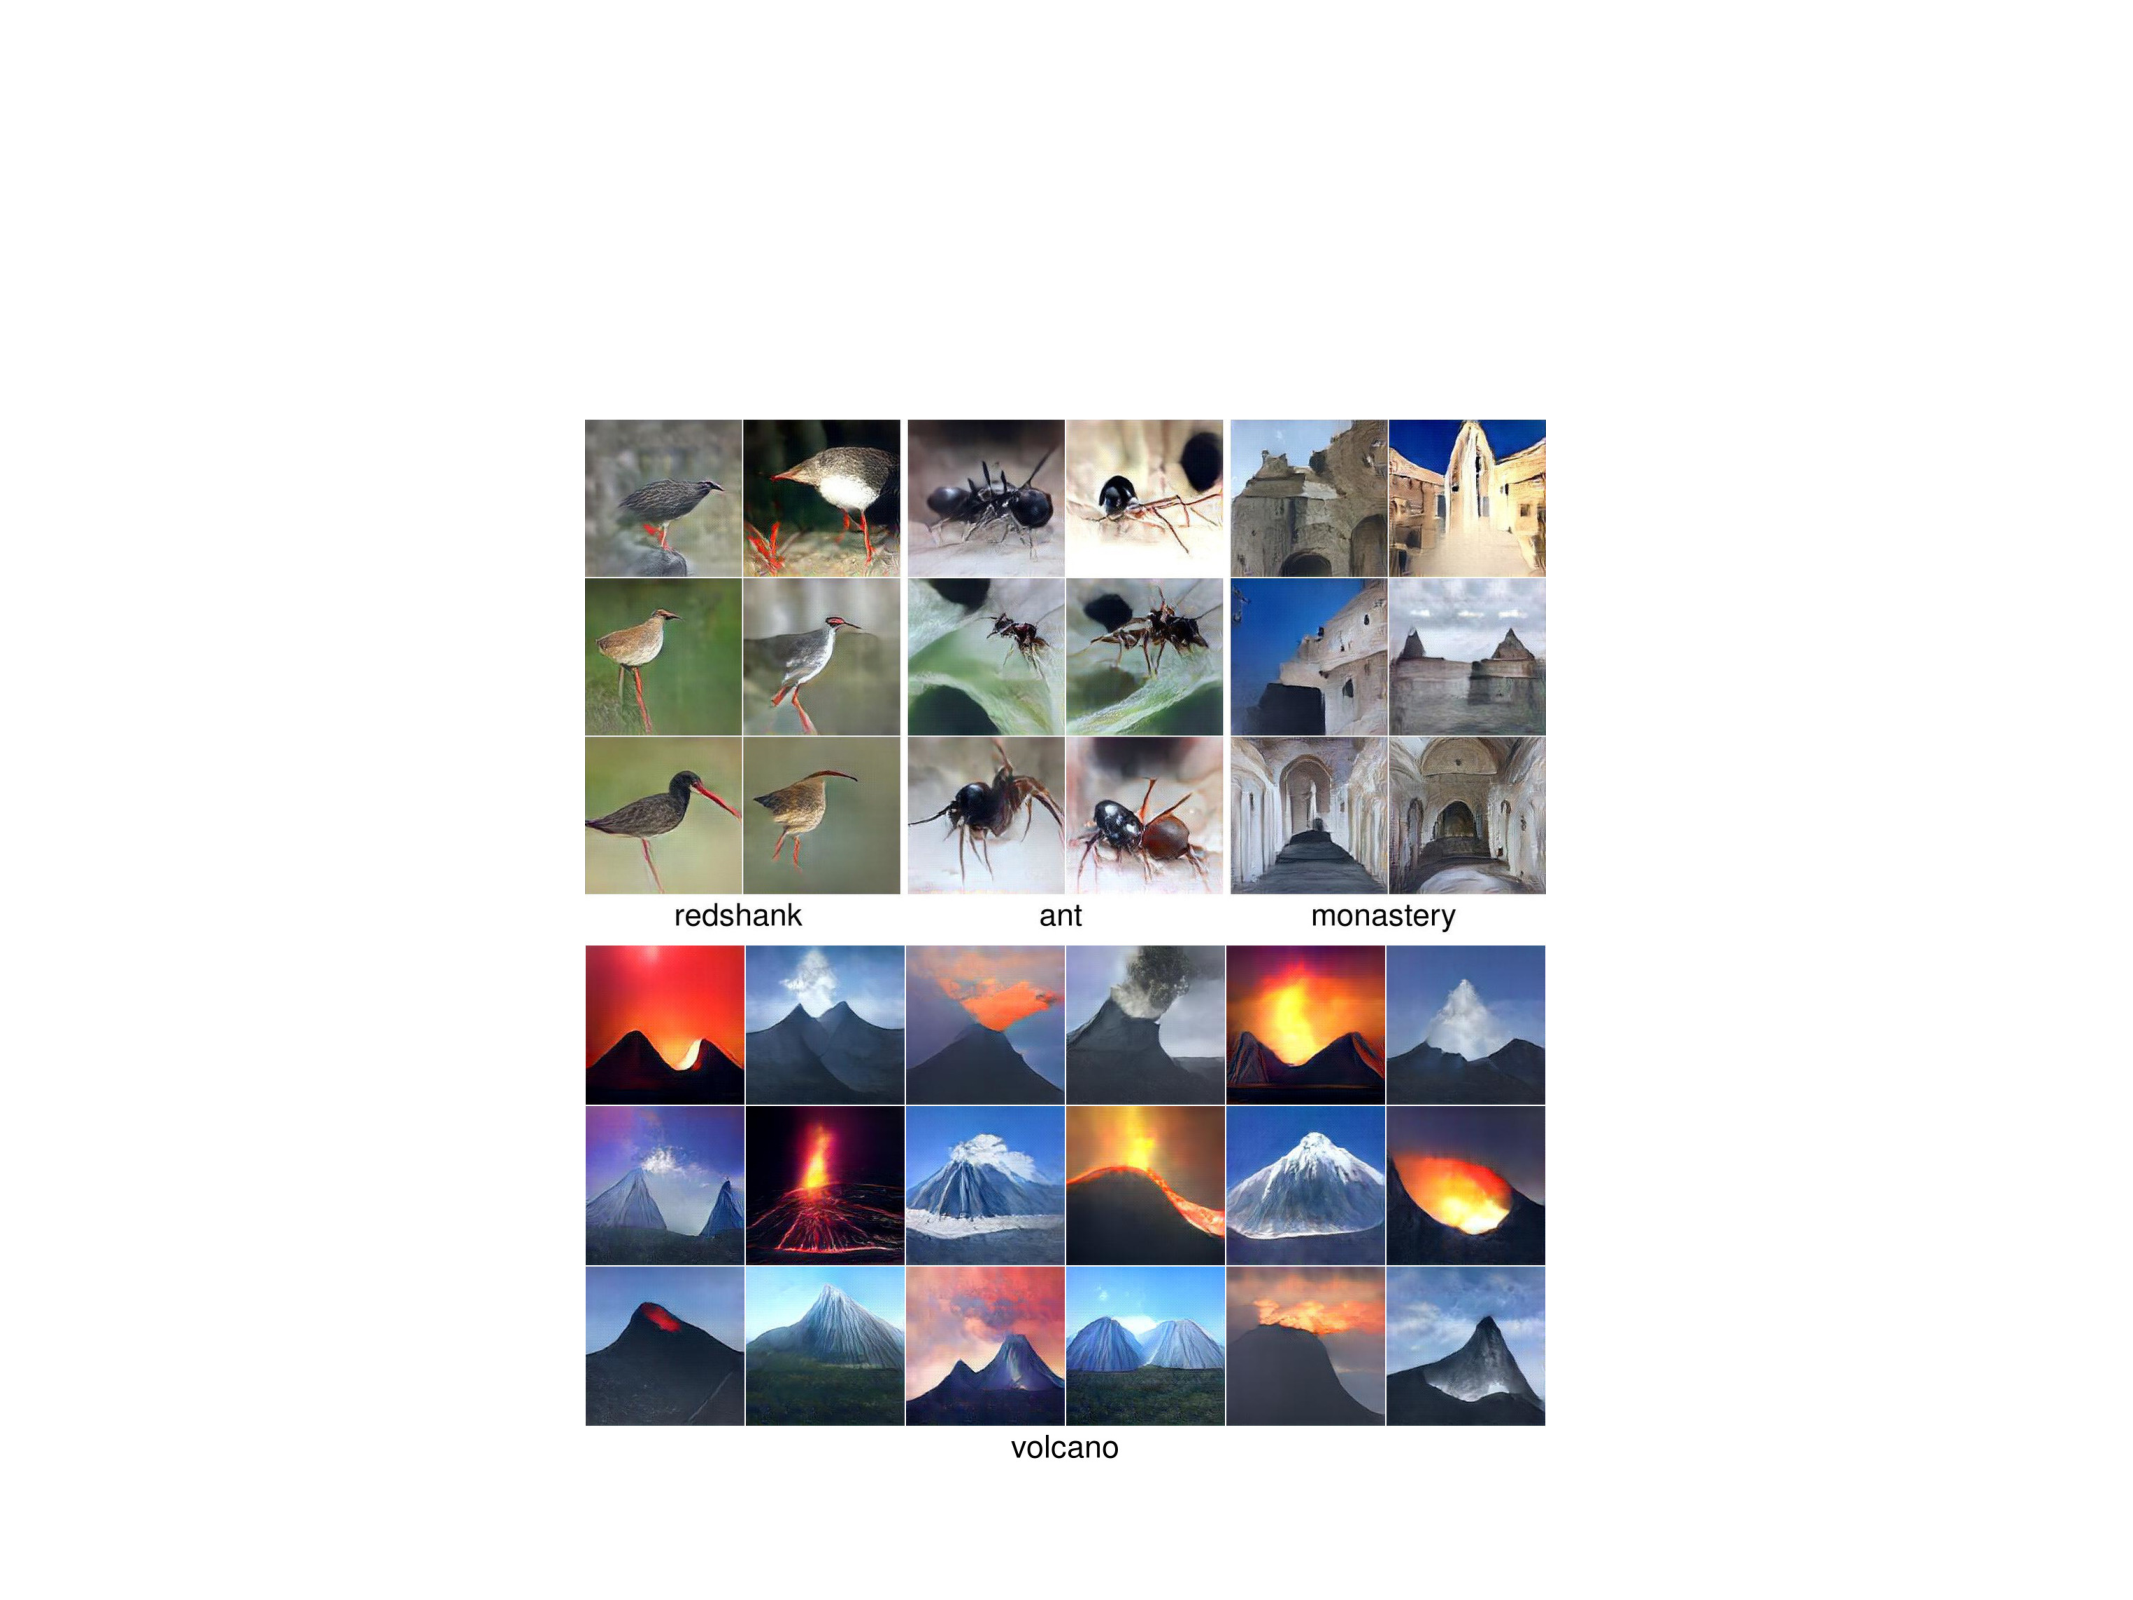
\includegraphics[width=\figwidth]{ppgn}
\caption{PPGNs are able to generate diverse, high resolution images from ImageNet
classes. Image reproduced from \citet{nguyen2016plug}.}
\label{fig:ppgn}
\end{figure}


\begin{figure}
\centering
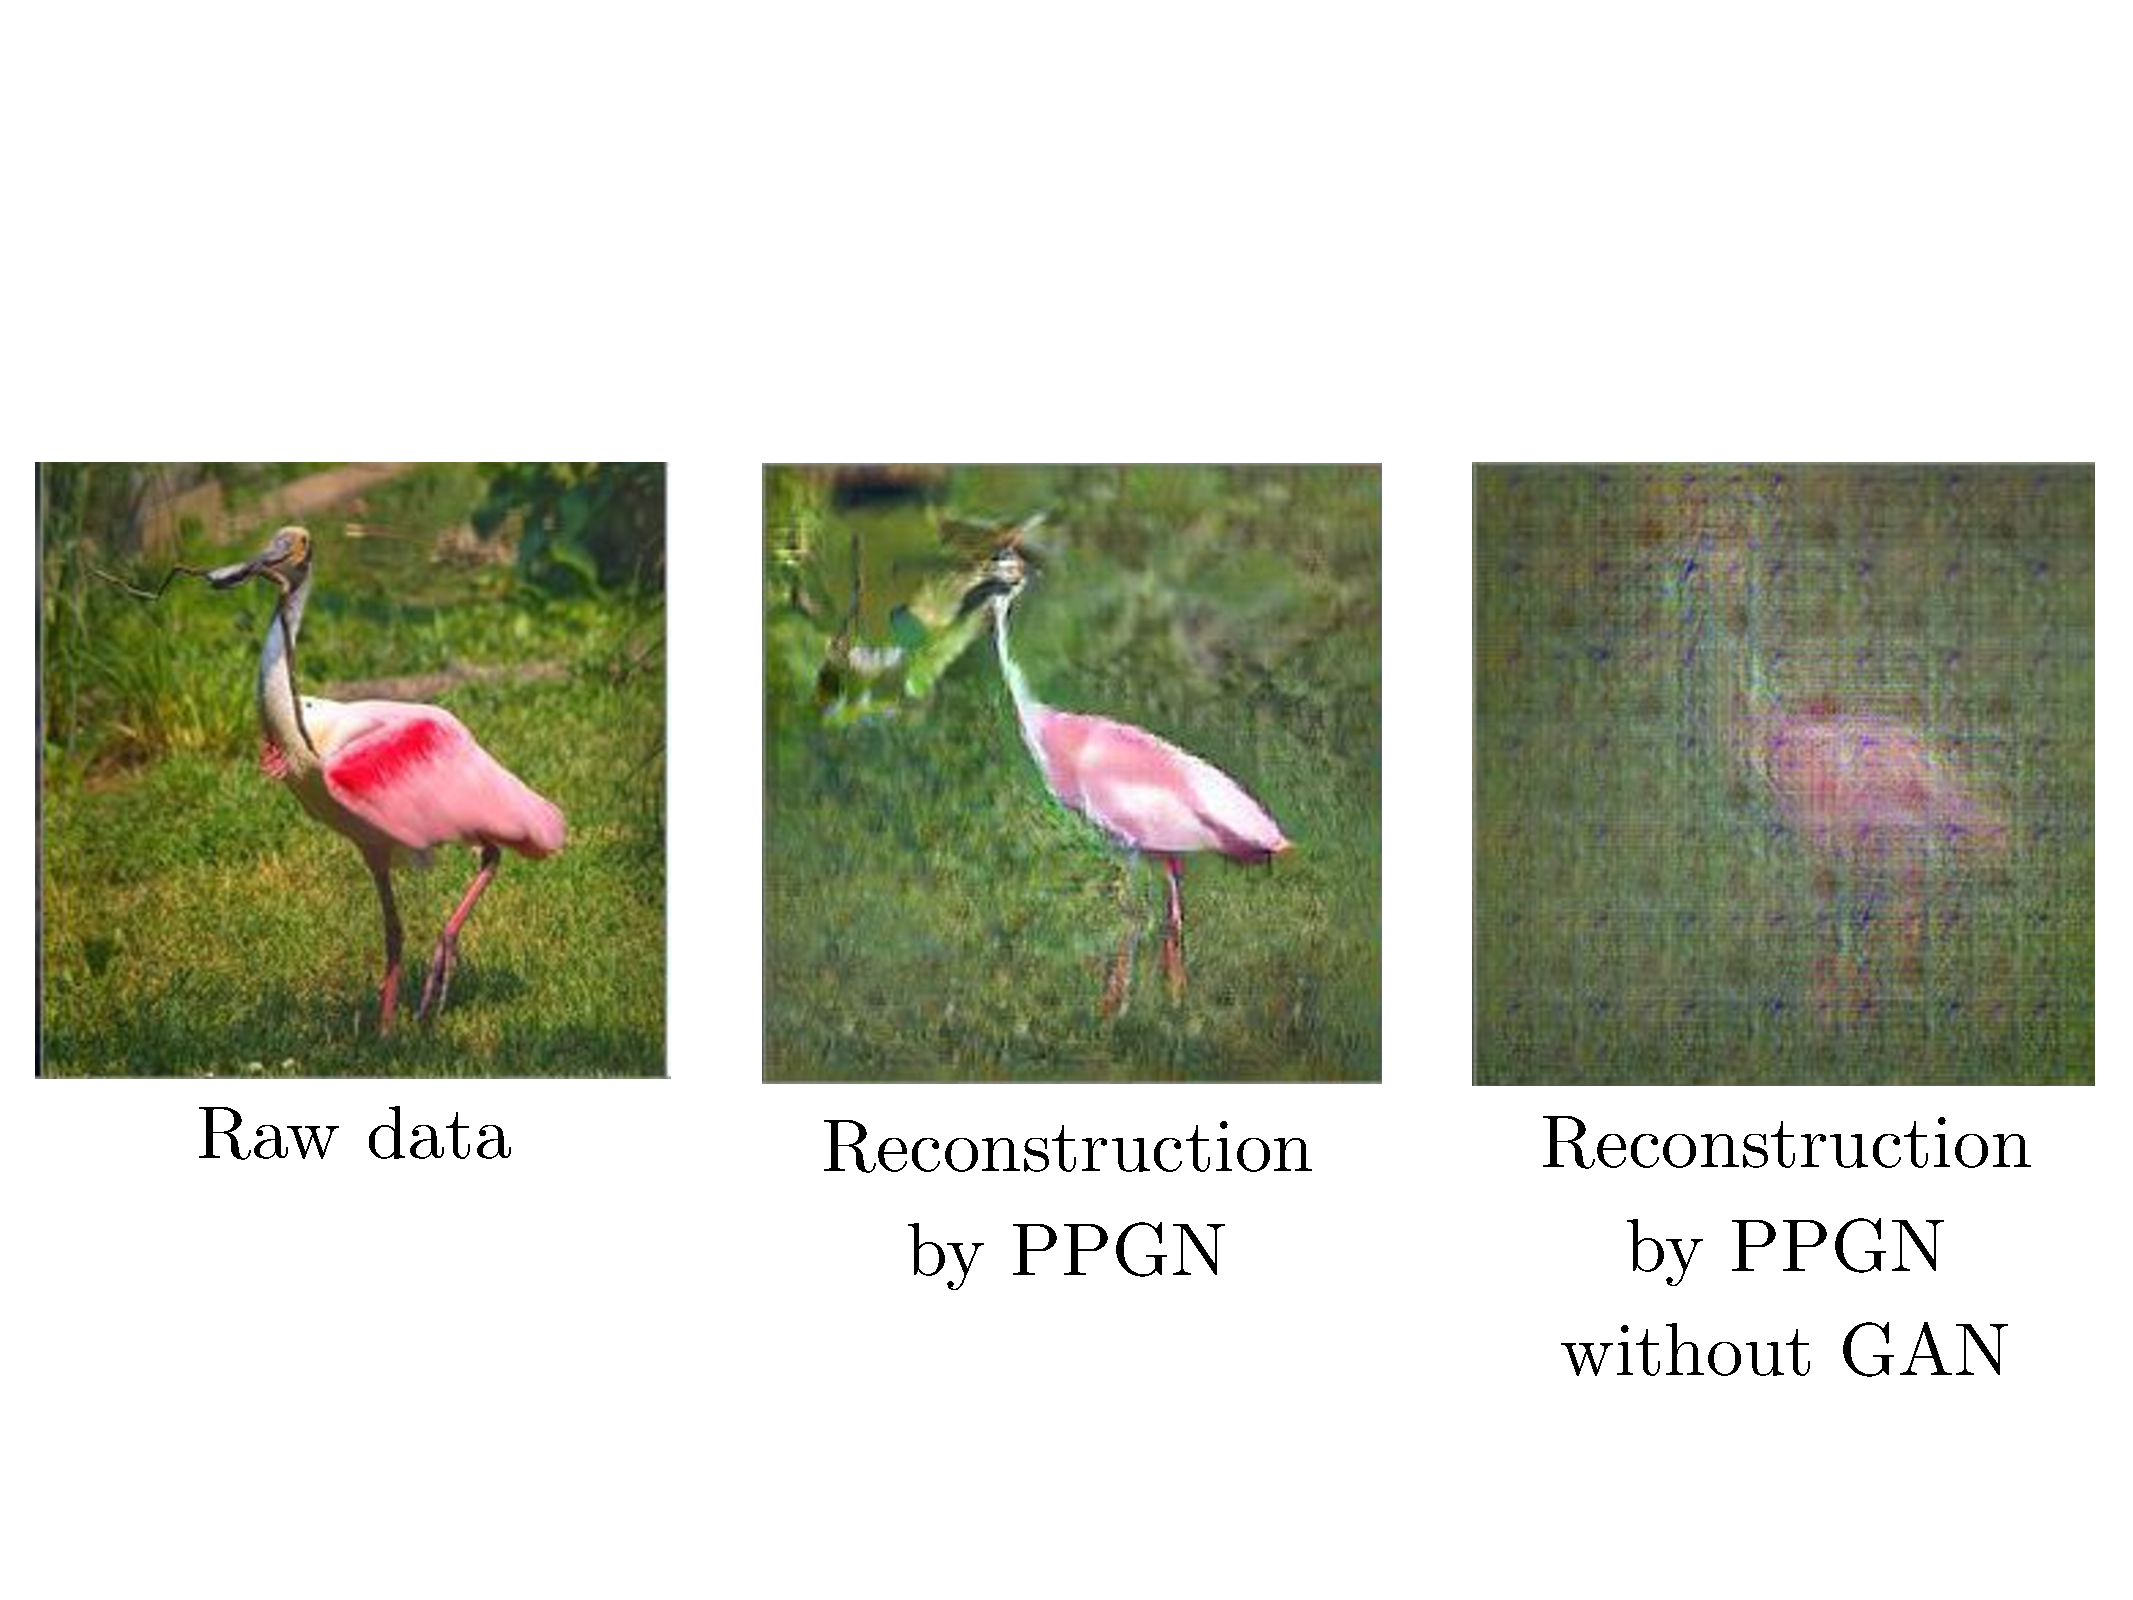
\includegraphics[width=\figwidth]{recons}
\caption{The GAN loss is a crucial ingredient of PPGNs. Without it, the denoising autoencoder
used to drive PPGNs does not create compelling images.}
\label{fig:recons}
\end{figure}


